\documentclass{article}

\PassOptionsToPackage{numbers,compress}{natbib}
% AI4DD is a double-blind workshop; \workshoptitle sets the submission footnote.
\usepackage[dblblindworkshop]{neurips_2026}
\workshoptitle{AI for Drug Discovery: Bridging the Translation Gap}
% The style only prints \workshoptitle in `final' mode, so the submission
% footnote is overridden here per the AI4DD call for papers.
\makeatletter
\renewcommand{\@noticestring}{%
  Submitted to the AI for Drug Discovery workshop (NeurIPS 2026). Do not distribute.%
}
\makeatother

\usepackage[utf8]{inputenc}
\usepackage[T1]{fontenc}
% BasicTeX ships Times (ptm) but not Courier (pcr); Latin Modern Mono is always
% present and avoids the missing-pcrr8t font error.
\renewcommand{\ttdefault}{lmtt}
\usepackage{amsmath,amssymb}
\usepackage{graphicx}
\usepackage{booktabs}
\usepackage{caption}
\usepackage{xcolor}
\usepackage{tikz}
\usetikzlibrary{arrows.meta,positioning,shapes.geometric}
\usepackage[colorlinks=true,allcolors=blue!60!black]{hyperref}
\usepackage{url}

\newcommand{\ddg}{\ensuremath{\Delta\Delta G}}
\newcommand{\rhoo}{\ensuremath{\rho}}
\newcommand{\kcal}{\,kcal/mol}

\title{When Structure Helps: Target-Dependent Docking and\\
Prior-Dependent Explanation for HIV Drug-Resistance Triage}

% Double-blind submission: the neurips_2026 style renders "Anonymous Author(s)"
% automatically. Restore the block below only for the camera-ready (final option).
% \author{%
%   Shreyash Goli \\
%   University of California, Berkeley \\
%   \texttt{shreyash\_goli@berkeley.edu}
% }

\begin{document}
\maketitle

\begin{abstract}
Antiviral drug resistance forces medicinal chemists to triage candidate inhibitors by how well their binding survives known resistance mutations---a slow, manual judgment. We present \textbf{ResistScope}, a target-agnostic pipeline that docks a candidate against a wildtype receptor plus a panel of clinical resistance mutants, scores binding robustness (\ddg), and generates a per-mutation mechanistic explanation with an LLM. Rather than report a single headline number, we ask two questions with real ground truth. \emph{First, does the docking score predict measured fold-resistance?} Across HIV-1 protease (6 protease inhibitors) and reverse transcriptase (4 NNRTIs) using Stanford HIVdb data, the answer is \textbf{target-dependent}: rigid single-structure \ddg{} is a chance-level ranker for the flexible, network-driven protease active site (ROC-AUC 0.51 [0.46, 0.56], below a zero-cost mutation-prevalence baseline of 0.72), but a moderate, genuinely above-chance one for the rigid, contact-driven NNRTI pocket (DRM enrichment $8.35\times$, ROC-AUC 0.70 [0.62, 0.77]; de-confounded single-mutation Spearman $\rhoo = 0.36$ [0.12, 0.56]). \emph{Second, do the explanations reflect real biology?} An LLM judge, scoring against IAS-USA and agentically-curated PubMed mechanisms, marks 71--72\% as recovering the correct primary mechanism (a judge-dependent absolute; the ablation contrasts are judge-robust across three models). An \textbf{attribution ablation} (real vs.\ absent vs.\ corrupted structural context) shows the explanations genuinely condition on the pipeline; across both targets the structural context's benefit \textbf{scales inversely with the model's prior knowledge}, and a field-level ablation suggests the benefit is localized to the mutation's \emph{geometry} (ligand distance, subpocket) rather than the docking energy. Taken together, these two contrasting targets support a hypothesis worth testing more broadly: structure-based methods, predictive and interpretive, deliver value precisely where non-structural shortcuts fail.
\end{abstract}

\section{Introduction}
Resistance is the central failure mode of antiviral therapy. A medicinal chemist with twenty candidate inhibitors must decide which few to advance into slow, expensive phenotypic resistance assays---a decision currently made by hand, mutation by mutation. A natural computational aid is to dock each candidate against a panel of known clinical resistance mutants and rank candidates by how well predicted binding \emph{survives} the panel.

Such a tool raises two questions that are usually asked separately, and that both have ground truth:
\begin{enumerate}
\item \textbf{Does the prediction hold up?} Stanford HIVdb records \emph{measured} fold-resistance for essentially every approved HIV drug \citep{rhee2006}. This turns ``is the score reasonable?'' into ``does the score predict a measured number, and does it beat the trivial baselines a chemist could use instead?''
\item \textbf{Does the \emph{explanation} hold up?} If the tool also explains \emph{why} a mutation threatens a compound, that explanation can be checked against mechanisms experts have already documented. Most structure-based resistance work never asks whether the model's \emph{reasoning}---not just its score---matches known biology.
\end{enumerate}

Our central observation, across both questions, is that \textbf{structure-based methods pay off exactly where the non-structural shortcut fails}. For prediction, the shortcut is mutation prevalence or an expert rule-base; structure adds value only for targets whose resistance is structurally local. For explanation, the shortcut is the LLM's memorized biology; structure adds value only for mutations the model has not memorized.

\textbf{Contributions.} (i) An honest, two-target benchmark of single-structure docking-\ddg{} for HIV resistance with significance-tested baselines, showing the method's value is \emph{target-dependent}. (ii) A faithfulness evaluation of the LLM's mechanistic explanations against expert and agentic ground truth. (iii) An attribution ablation isolating whether faithfulness comes from the structural pipeline or the model's prior, revealing a \emph{prior-strength dose-response} and localizing the effect to geometry. (iv) A reproducible, target-agnostic implementation (protease, RT, bring-your-own-target).

\begin{figure}[t]
\centering
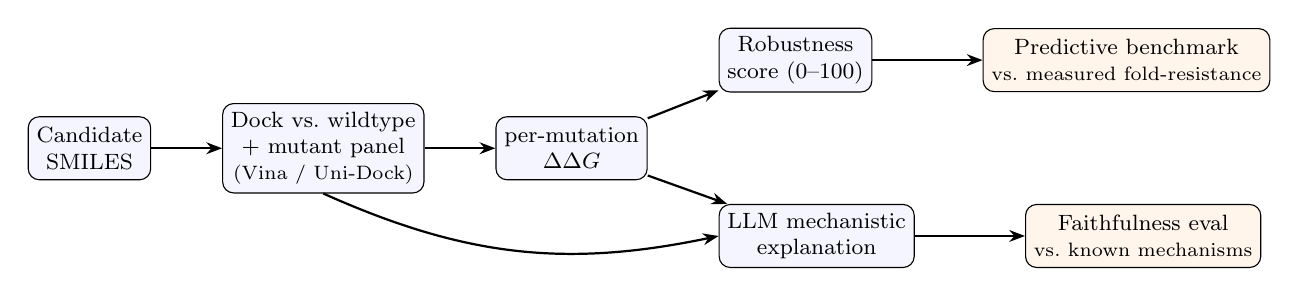
\begin{tikzpicture}[
  node distance=6mm and 9mm,
  box/.style={draw, rounded corners, align=center, font=\footnotesize, minimum height=8mm, inner sep=3pt, fill=blue!4},
  val/.style={draw, rounded corners, align=center, font=\footnotesize, minimum height=8mm, inner sep=3pt, fill=orange!8},
  ar/.style={-{Stealth[length=2mm]}, thick}]
  \node[box] (smi) {Candidate\\SMILES};
  \node[box, right=of smi] (dock) {Dock vs.\ wildtype\\$+$ mutant panel\\{\scriptsize (Vina / Uni-Dock)}};
  \node[box, right=of dock] (ddg) {per-mutation\\\ddg};
  \node[box, above right=3mm and 9mm of ddg] (score) {Robustness\\score (0--100)};
  \node[box, below right=3mm and 9mm of ddg] (expl) {LLM mechanistic\\explanation};
  \node[val, right=14mm of score] (pred) {Predictive benchmark\\{\scriptsize vs.\ measured fold-resistance}};
  \node[val, right=14mm of expl] (faith) {Faithfulness eval\\{\scriptsize vs.\ known mechanisms}};
  \draw[ar] (smi) -- (dock);
  \draw[ar] (dock) -- (ddg);
  \draw[ar] (ddg) -- (score);
  \draw[ar] (ddg) -- (expl);
  \draw[ar] (score) -- (pred);
  \draw[ar] (expl) -- (faith);
  \draw[ar] (dock.south) to[bend right=18] (expl.west);
\end{tikzpicture}
\caption{\textbf{ResistScope pipeline.} A candidate SMILES is docked against the wildtype receptor and a panel of clinical resistance mutants; per-mutation \ddg{} yields a robustness score and, with structural context, an LLM mechanistic explanation. Each output is validated against real ground truth: predicted \ddg{} against measured fold-resistance, and explanations against documented mechanisms.}
\label{fig:pipeline}
\end{figure}

\section{Related work}

\textbf{Rule-based expert systems} are the clinical standard for interpreting HIV resistance genotypes and are our strongest baseline. The Stanford HIVdb penalty algorithm \citep{liu2006,rhee2006} and the IAS-USA mutation lists \citep{iasusa} encode decades of accumulated genotype--phenotype and clinical-outcome evidence into per-mutation, per-drug scores. They are accurate precisely because that evidence exists; they say nothing about a compound or target for which it does not.

\textbf{Supervised ML on genotype--phenotype data} is the dominant computational approach and reaches high retrospective accuracy. \texttt{geno2pheno} learns decision trees and SVMs mapping sequence to phenotypic resistance \citep{beerenwinkel2003}; deep architectures (MLP, bidirectional RNN, CNN) have been trained across 18 antiretrovirals \citep{steiner2020}; large-scale gradient boosting and random forests over clinical sequence corpora recover both known and novel resistance mutations \citep{blassel2021}; and protein language-model embeddings now push mean AUC to $\approx0.97$ \citep{farquhar2026}. These are strong, obvious baselines, and we do not claim to beat them. They share one structural requirement that motivates our work: each needs a labeled resistance dataset \emph{for the drug in question}. Docking is training-free, so it is applicable exactly where these methods are not---a novel scaffold, or a target with no resistance corpus. Our study asks whether that applicability is worth anything, and finds the answer depends on the target.

\textbf{Structure-based resistance prediction} has a long history and an established explanation for why protease is hard. The substrate-envelope hypothesis \citep{king2004,nalam2010} holds that protease resistance mutations selectively disrupt inhibitor binding at positions where the inhibitor protrudes beyond the consensus substrate volume, while leaving substrate processing intact---a coevolutionary, network-level constraint that a single-structure pocket-affinity score is not designed to capture. This predicts our protease result. Other structure-aware approaches include molecular field mapping over homology models \citep{ota2021} and, at the accurate-but-expensive end, alchemical free-energy calculations, which reach 88\% accuracy on 144 clinical Abl kinase mutations at roughly 1.1\kcal{} RMSE \citep{hauser2018}---orders of magnitude more compute per mutation than rigid docking. Receptor flexibility is the standard remedy for rigid-docking failure, via ensemble or relaxed-complex schemes \citep{amaro2008}; we do not employ it, which bounds how far our negative protease result generalizes. Learned co-folding and affinity models are a rapidly moving alternative \citep{boltz2}, though careful benchmarking shows deep docking methods can produce physically invalid poses and generalize poorly off-distribution \citep{posebusters}.

\textbf{LLM explanation faithfulness.} Whether a model's stated reasoning reflects the computation that produced its answer is a distinct question from whether the answer is right \citep{jacovi2020}. Chain-of-thought rationales can be systematically \emph{plausible but unfaithful}, rationalizing answers driven by features the model never mentions \citep{turpin2023}. LLM-as-judge evaluation is now standard and correlates well with human preference, but carries known biases that make absolute scores judge-dependent \citep{zheng2023}---which is why we report cross-model judge agreement and rest our claims on paired within-judge contrasts. Our corrupted-context condition follows the ablation logic of Min et al.~\citep{min2022}, who showed that replacing in-context labels with random ones barely degrades performance, implying the model was not conditioning on them; we apply the same test to structural context. LLMs are increasingly deployed as tool-using agents in chemistry \citep{chemcrow}, but the faithfulness of their domain-specific mechanistic claims is rarely measured; that gap is our second contribution.

\section{Methods}
\textbf{Pipeline.} A candidate SMILES is embedded (RDKit/meeko) and docked (AutoDock Vina \citep{vina} on CPU, or Uni-Dock \citep{unidock} on GPU) against a cleaned wildtype receptor and a per-drug panel of point-mutant receptors; the per-mutation \ddg{} (mutant minus wildtype binding) feeds a 0--100 robustness score. Mutant receptors are built by PDBFixer point mutagenesis with a frozen-environment clash-relief minimization of the mutated side chain. We note throughout that the Vina score is an empirical scoring function, not a binding free energy; we use it as a ranking signal only.

\textbf{Targets and data.} \emph{Protease} (PR): PDB 3OXC, homodimer, catalytic Asp25 dyad asymmetrically protonated; 6 PIs; 285 mutant receptors; 1{,}591 drug--mutation pairs. \emph{Reverse transcriptase} (RT): PDB 3V81, p66/p51 heterodimer, NNRTI-pocket docking box on the chain-A nevirapine ligand; 4 NNRTIs; 424 mutant receptors; 1{,}269 pairs. We scope RT to NNRTIs (allosteric pocket binders): rigid docking is a sound proxy for NNRTI affinity but not for NRTI mechanisms. Measured fold-resistance and DRM labels come from Stanford HIVdb / IAS-USA \citep{rhee2006,iasusa}.

\textbf{Explanations and ground truth.} For each mutation we assemble a structural-context record (residue identity, $\Delta$volume/charge/hydrophobicity, ligand distance, direct-contact flag, subpocket) plus the docking \ddg, and prompt an LLM (Claude Haiku 4.5; larger models decline HIV-resistance \emph{generation}, though not judging) for a 2--3 sentence mechanistic hypothesis. Ground truth combines a curated set (IAS-USA $+$ primary literature) with an \emph{agentic} builder that researches each mechanism over live PubMed, cites the papers, and self-verifies grounding. All RT ground truth is agent-built; PR ground truth is hand-curated, so we lead the faithfulness headline with PR.

\textbf{Faithfulness and attribution.} An LLM-as-judge scores each explanation against the ground-truth mechanism on a 0/1/2 rubric; we assess judge robustness with independent models (\S\ref{sec:faith}). The attribution ablation regenerates explanations under \emph{full} (real context $+$ \ddg), \emph{minimal} (drug $+$ mutation only), and \emph{corrupted} (pipeline-derived fields deranged across pairs, intrinsic chemistry kept) conditions with the same model and judge; a field-level variant drops one context group at a time.

\textbf{Predictive benchmark.} Every claim carries a permutation $p$-value or bootstrap 95\% CI: top-$N$ DRM enrichment, threshold-free ROC/PR-AUC, a de-confounding analysis (rebuild the fold-resistance target from progressively less co-mutated isolate subsets), a leave-one-drug-out jackknife, and baselines (mutation prevalence, physicochemical $|\Delta\text{volume}|$, and the Stanford HIVdb penalty score via the Sierra GraphQL API). We report many tests and apply no multiplicity correction; the headline contrasts survive at $p<10^{-3}$, but marginal $p$-values should be read accordingly.

\section{Results}

\subsection{The predictive benchmark is target-dependent}
Rigid single-structure docking-\ddg{} behaves oppositely on the two enzymes (Fig.~\ref{fig:benchmark}, Appendix~\ref{app:benchmark}).

\textbf{Protease---chance-level, loses to trivial baselines.} Top-40 DRM enrichment is $2.86\times$ (95\% CI 1.63--4.08, $p<0.001$), but pooled DRM-recovery ROC-AUC is only 0.51 [0.46, 0.56] and per-mutation Spearman with measured fold-resistance is $\approx 0$. De-confounding does \emph{not} rescue it ($\rhoo \leq 0$). Extreme-tail enrichment and chance-level global ranking are not contradictory: the method's most confident predictions are enriched for real DRMs even though it orders the full list no better than chance.

\textbf{RT---a genuine ranker, and de-confounding rescues.} Top-40 enrichment is $8.35\times$ (95\% CI 6.7--9.7); pooled ROC-AUC is 0.70 [0.62, 0.77], a moderate but reliably above-chance value; and the pooled magnitude correlation goes from $-0.11$ (confounded) to $\rhoo = 0.36$ [0.12, 0.56] ($p=6\times10^{-4}$, leave-one-out range [0.34, 0.40]) on single-mutation isolates---the co-mutation confound was masking a real single-mutation signal. Wildtype affinities ($-9$ to $-12$\kcal) confirm the docking box is on the pocket.

\begin{table}[t]
\centering
\caption{\textbf{Baseline head-to-head.} DRM-recovery ROC-AUC / magnitude Spearman \rhoo{} vs.\ measured fold-resistance. HIVdb (expert system) wins both; docking never beats it retrospectively, but requires no clinical or expert data for the compound in question. (Bootstrap 95\% CIs in text; HIVdb's ROC is partly circular vs.\ the expert DRM labels, so \rhoo{} is the fair column.)}
\label{tab:baselines}
\begin{tabular}{lcc}
\toprule
predictor & protease (ROC / \rhoo) & RT (ROC / \rhoo) \\
\midrule
docking \ddg{}        & 0.51 / 0.00 & \textbf{0.70} / $-0.11$ {\scriptsize(de-conf.\ $+0.36$)} \\
mutation prevalence   & 0.72 / $-0.08$ & 0.65 / 0.13 \\
$|\Delta\text{volume}|$ & 0.49 / 0.14 & 0.65 / $-0.01$ \\
\textbf{HIVdb penalty} & \textbf{0.86 / 0.36} & \textbf{0.93 / 0.27} \\
\bottomrule
\end{tabular}
\end{table}

The expert system (HIVdb) is strongest on both, and \textbf{docking never beats it retrospectively} (Table~\ref{tab:baselines}): on protease docking loses even to zero-cost prevalence; on RT it beats the docking-free baselines but not HIVdb. A leave-one-drug-out jackknife confirms the pattern is not driven by any single drug (protease ROC range [0.50, 0.53]; RT [0.67, 0.74]).

\textbf{The metric the chemist actually uses.} ROC-AUC scores a full ranking, but the tool is read as the top few flagged mutations for \emph{one} compound. Per-drug precision@$k$ (Appendix~\ref{app:perdrug}) turns the same contrast into a decision-relevant number: for every NNRTI, 7--8 of the top 10 flagged mutations are genuine clinical DRMs (median precision@10 $=0.75$ vs.\ base rates 0.07--0.20, all four $p<0.001$), whereas the PI median is 0.20 against a 0.12 base rate and indinavir's top 10 contain none. The deployed ranking is useful---on exactly one of the two targets.

\textbf{Why the difference.} NNRTIs bind a compact, rigid pocket where resistance is direct steric/contact disruption---what rigid \ddg{} captures. Protease resistance is flexible-active-site, co-evolving, and substrate-envelope-constrained \citep{king2004,nalam2010}---what rigid docking misses. \emph{Why docking might still be worth running} is a hypothesis rather than a result of this paper: the baselines that beat docking (prevalence, HIVdb, supervised ML) all require clinical or expert data that a novel compound or novel target does not have, whereas docking requires none. We flag this as our motivation, not a validated finding; the per-drug ROC on RT (0.63--0.77) is the nearest evidence we have, and a scaffold-holdout test is the experiment that would settle it.

\subsection{Explanation faithfulness}
\label{sec:faith}
Under the Claude-Haiku judge, explanations recover the correct primary mechanism 72\% of the time on protease ($n=46$, hand-curated ground truth) and 71\% on RT ($n=55$, agent-built ground truth, so its absolute value is the weaker of the two); most misses under-specify rather than contradict. On RT the outright misses cluster on distal/allosteric DRMs---for example the E138--K101 inter-subunit salt bridge that couples the p51 and p66 subunits \citep{das2013}, and A98G---where single-structure docking is genuinely blind, and the model faithfully reports ``no direct effect.''

\textbf{Judge robustness (cross-model).} Two checks. On a 21-item sample stratified to over-represent the judge's hard (0/1) cases, GPT-5.6 agrees with Claude-Haiku 95\% within one point but only 48\% exactly (Cohen's $\kappa$ 0.23 unweighted, 0.38 linear-weighted); Claude is systematically \emph{stricter}. Critically, re-grading all 138 protease ablation items with a \emph{second} Claude model (Sonnet 5) reproduces the \S\ref{sec:abl} contrasts almost exactly (full$-$minimal $\Delta=+0.35$, $p=0.001$; full$-$corrupted $\Delta=+0.65$, $p<10^{-4}$, vs.\ Haiku's $+0.43/+0.63$; Sonnet--Haiku $\kappa=0.64/0.72$, within-1 100\%). Consistent with known judge biases \citep{zheng2023}, we therefore treat the \emph{absolute} faithfulness percentage as judge-dependent and rest our claims on the \emph{paired within-judge} contrasts of \S\ref{sec:abl}, which are judge-robust. All three judges are LLMs; a human-expert anchor remains future work and is the single most valuable addition to this evaluation.

\subsection{Attribution ablation: the pipeline drives faithfulness, geometrically, where the prior is weak}
\label{sec:abl}
\textbf{Context is genuinely used.} Pooled across both targets ($n=101$), full context beats minimal (drug $+$ mutation only) by $\Delta=+0.27$ ($p=7\times10^{-4}$) and beats corrupted context by $\Delta=+0.46$ ($p<10^{-4}$). Feeding \emph{wrong} structural facts is worse than feeding none---by the logic of Min et al.~\citep{min2022}, the explanations are conditioning on the pipeline rather than pattern-matching the mutation name (Fig.~\ref{fig:interp}a, Appendix~\ref{app:interp}).

\textbf{Prior-strength dose-response.} The benefit of correct context scales inversely with the model's prior (Fig.~\ref{fig:interp}b). Where the prior alone is \emph{wrong} (minimal $=0$, $n=13$), context corrects the explanation in 11 of 13 cases (85\%); where vague (minimal $=1$), 66\%; where already correct (minimal $=2$), context is at ceiling. Because the raw gain is partly mechanical---a score of 0 has twice the headroom of a 1---we lead with these ceiling-robust improvement rates. Restricting to pairs with room to improve (minimal $<2$, $n=45$), context still helps $\Delta=+0.80$ ($p<10^{-4}$) and the gradient persists (Spearman $\rhoo=-0.40$, $p=0.006$), so the effect is not headroom alone.

\textbf{Geometry, not energy.} A field-level ablation (protease, $n=46$; Fig.~\ref{fig:interp}c) drops one context group at a time. Removing the \emph{ligand distance} costs the most ($\Delta=+0.22$, $p=0.051$) and the \emph{subpocket} next ($\Delta=+0.15$, $p=0.09$); removing the \emph{docking \ddg} ($\Delta=-0.02$) or the physicochemistry ($\Delta=-0.02$) does nothing measurable. This suggests---at marginal significance, on one target, $n=46$---that the pipeline's explanatory value is its geometric localization of the mutation rather than its energy term. The null on \ddg{} is absence of evidence, and it is specifically a null for \emph{rigid, single-pose, waters-stripped Vina} \ddg{}: a more accurate energy (ensemble docking \citep{amaro2008}, free-energy calculation \citep{hauser2018}) might well contribute where ours does not. Replication on RT and on the low-prior subset is the natural next step.

\section{Discussion}
The two findings share one account: \textbf{structure-based methods deliver value where the non-structural shortcut fails.} For prediction, the shortcut is prevalence, expert rules, or supervised ML, and structure helps only when resistance is structurally local (the NNRTI pocket, not the protease active site). For explanation, the shortcut is the LLM's parametric biology, and structure helps only for mutations the model has not memorized---through the mutation's \emph{geometry}. We offer this as a hypothesis supported by two deliberately contrasting targets, not a law: both are HIV enzymes, and confirming it requires more targets of differing pocket biophysics. Read as a practical rule of thumb, it says: expect structure-based resistance triage to work for rigid, contact-driven pockets and single-mutation regimes, distrust it for flexible, allosteric, co-evolving sites, and reach for it in the prospective setting where clinical and expert baselines do not yet exist---the setting a scaffold-holdout experiment should test next.

\textbf{Limitations.} Every claim about docking \emph{energy} is bounded by the protocol: rigid single-structure Vina, no ensemble or flexible receptor, crystal waters (including the conserved flap water) stripped, and the score read as a ranking signal rather than a free energy. RT ground truth is agent-built and needs a human-expert anchor; the judge's absolute scores are judge-dependent ($\kappa\approx0.23$--0.38 cross-vendor on hard cases, 0.64--0.72 cross-model) though the paired contrasts reproduce. Per-bin $n$ is modest and many tests carry no multiplicity correction. Precision@$k$ validates the \emph{ranking} the robustness score induces, but with 6$+$4 compounds its absolute 0--100 calibration is untested, so all quantitative validation here is per-mutation.

\bibliographystyle{plainnat}
\begin{thebibliography}{99}

\bibitem{amaro2008} Amaro, R.~E., Baron, R., McCammon, J.~A. An improved relaxed complex scheme for receptor flexibility in computer-aided drug design. \emph{Journal of Computer-Aided Molecular Design}, 2008.

\bibitem{beerenwinkel2003} Beerenwinkel, N., D\"aumer, M., Oette, M., Korn, K., Hoffmann, D., Kaiser, R., Lengauer, T., Selbig, J., Walter, H. Geno2pheno: estimating phenotypic drug resistance from HIV-1 genotypes. \emph{Nucleic Acids Research}, 31(13):3850--3855, 2003.

\bibitem{blassel2021} Blassel, L., Tostevin, A., Villabona-Arenas, C.~J., Peeters, M., Hu\'e, S., Gascuel, O. Using machine learning and big data to explore the drug resistance landscape in HIV. \emph{PLOS Computational Biology}, 17(8):e1008873, 2021.

\bibitem{boltz2} Passaro, S., et al. Boltz-2: Towards accurate and efficient binding affinity prediction. \emph{bioRxiv}, 2025. doi:10.1101/2025.06.14.659707.

\bibitem{chemcrow} M.\ Bran, A., Cox, S., Schilter, O., Baldassari, C., White, A.~D., Schwaller, P. Augmenting large language models with chemistry tools. \emph{Nature Machine Intelligence}, 6:525--535, 2024.

\bibitem{posebusters} Buttenschoen, M., Morris, G.~M., Deane, C.~M. PoseBusters: AI-based docking methods fail to generate physically valid poses or generalise to novel sequences. \emph{Chemical Science}, 15(9):3130--3139, 2024.

\bibitem{das2013} Das, K., Arnold, E. HIV-1 reverse transcriptase and antiviral drug resistance. Part 2. \emph{Current Opinion in Virology}, 2013.

\bibitem{vina} Eberhardt, J., Santos-Martins, D., Tillack, A.~F., Forli, S. AutoDock Vina 1.2.0: New docking methods, expanded force field, and Python bindings. \emph{Journal of Chemical Information and Modeling}, 61:3891--3898, 2021. See also Trott, O., Olson, A.~J., \emph{Journal of Computational Chemistry}, 31:455--461, 2010.

\bibitem{farquhar2026} Farquhar, H. Protein language model embeddings improve HIV drug resistance prediction: a comprehensive benchmark with attention-based interpretability. \emph{Bioinformatics}, 42(5):btag260, 2026.

\bibitem{hauser2018} Hauser, K., Negron, C., Albanese, S.~K., Ray, S., Steinbrecher, T., Abel, R., Chodera, J.~D., Wang, L. Predicting resistance of clinical Abl mutations to targeted kinase inhibitors using alchemical free-energy calculations. \emph{Communications Biology}, 1:70, 2018.

\bibitem{jacovi2020} Jacovi, A., Goldberg, Y. Towards faithfully interpretable NLP systems: How should we define and evaluate faithfulness? In \emph{Proceedings of ACL}, pp.\ 4198--4205, 2020.

\bibitem{king2004} King, N.~M., Prabu-Jeyabalan, M., Nalivaika, E.~A., Schiffer, C.~A. Combating susceptibility to drug resistance: lessons from HIV-1 protease. \emph{Chemistry \& Biology}, 2004.

\bibitem{liu2006} Liu, T.~F., Shafer, R.~W. Web resources for HIV type 1 genotypic-resistance test interpretation. \emph{Clinical Infectious Diseases}, 42(11):1608--1618, 2006.

\bibitem{min2022} Min, S., Lyu, X., Holtzman, A., Artetxe, M., Lewis, M., Hajishirzi, H., Zettlemoyer, L. Rethinking the role of demonstrations: What makes in-context learning work? In \emph{Proceedings of EMNLP}, 2022.

\bibitem{nalam2010} Nalam, M.~N.~L., Ali, A., Altman, M.~D., Reddy, G.~S.~K.~K., Chellappan, S., Kairys, V.,\"Ozen, A., Cao, H., Gilson, M.~K., Tidor, B., Rana, T.~M., Schiffer, C.~A. Evaluating the substrate-envelope hypothesis: structural analysis of novel HIV-1 protease inhibitors designed to be robust against drug resistance. \emph{Journal of Virology}, 84(10):5368--5378, 2010.

\bibitem{ota2021} Ota, R., So, K., Tsuda, M., Higuchi, Y., Yamashita, F. Prediction of HIV drug resistance based on the 3D protein structure: Proposal of molecular field mapping. \emph{PLOS ONE}, 2021. doi:10.1371/journal.pone.0255693.

\bibitem{rhee2006} Rhee, S.-Y., Taylor, J., Wadhera, G., Ben-Hur, A., Brutlag, D.~L., Shafer, R.~W. Genotypic predictors of human immunodeficiency virus type 1 drug resistance. \emph{PNAS}, 103(46):17355--17360, 2006. Stanford HIV Drug Resistance Database, \url{https://hivdb.stanford.edu}.

\bibitem{steiner2020} Steiner, M.~C., Gibson, K.~M., Crandall, K.~A. Drug resistance prediction using deep learning techniques on HIV-1 sequence data. \emph{Viruses}, 12(5):560, 2020.

\bibitem{turpin2023} Turpin, M., Michael, J., Perez, E., Bowman, S.~R. Language models don't always say what they think: Unfaithful explanations in chain-of-thought prompting. In \emph{Advances in Neural Information Processing Systems 36}, 2023.

\bibitem{iasusa} Wensing, A.~M., Calvez, V., Ceccherini-Silberstein, F., Charpentier, C., G\"unthard, H.~F., Paredes, R., Shafer, R.~W., Richman, D.~D. 2022 update of the drug resistance mutations in HIV-1. \emph{Topics in Antiviral Medicine}, 30(4):559--574, 2022.

\bibitem{unidock} Yu, Y., Cai, C., Wang, J., Bo, Z., Zhu, Z., Zheng, H. Uni-Dock: GPU-accelerated docking enables ultralarge virtual screening. \emph{Journal of Chemical Theory and Computation}, 2023.

\bibitem{zheng2023} Zheng, L., Chiang, W.-L., Sheng, Y., Zhuang, S., Wu, Z., Zhuang, Y., Lin, Z., Li, Z., Li, D., Xing, E.~P., Zhang, H., Gonzalez, J.~E., Stoica, I. Judging LLM-as-a-judge with MT-Bench and Chatbot Arena. In \emph{Advances in Neural Information Processing Systems 36}, 2023.

\end{thebibliography}

\appendix

\section{Predictive benchmark figures}
\label{app:benchmark}

\begin{figure}[h]
\centering
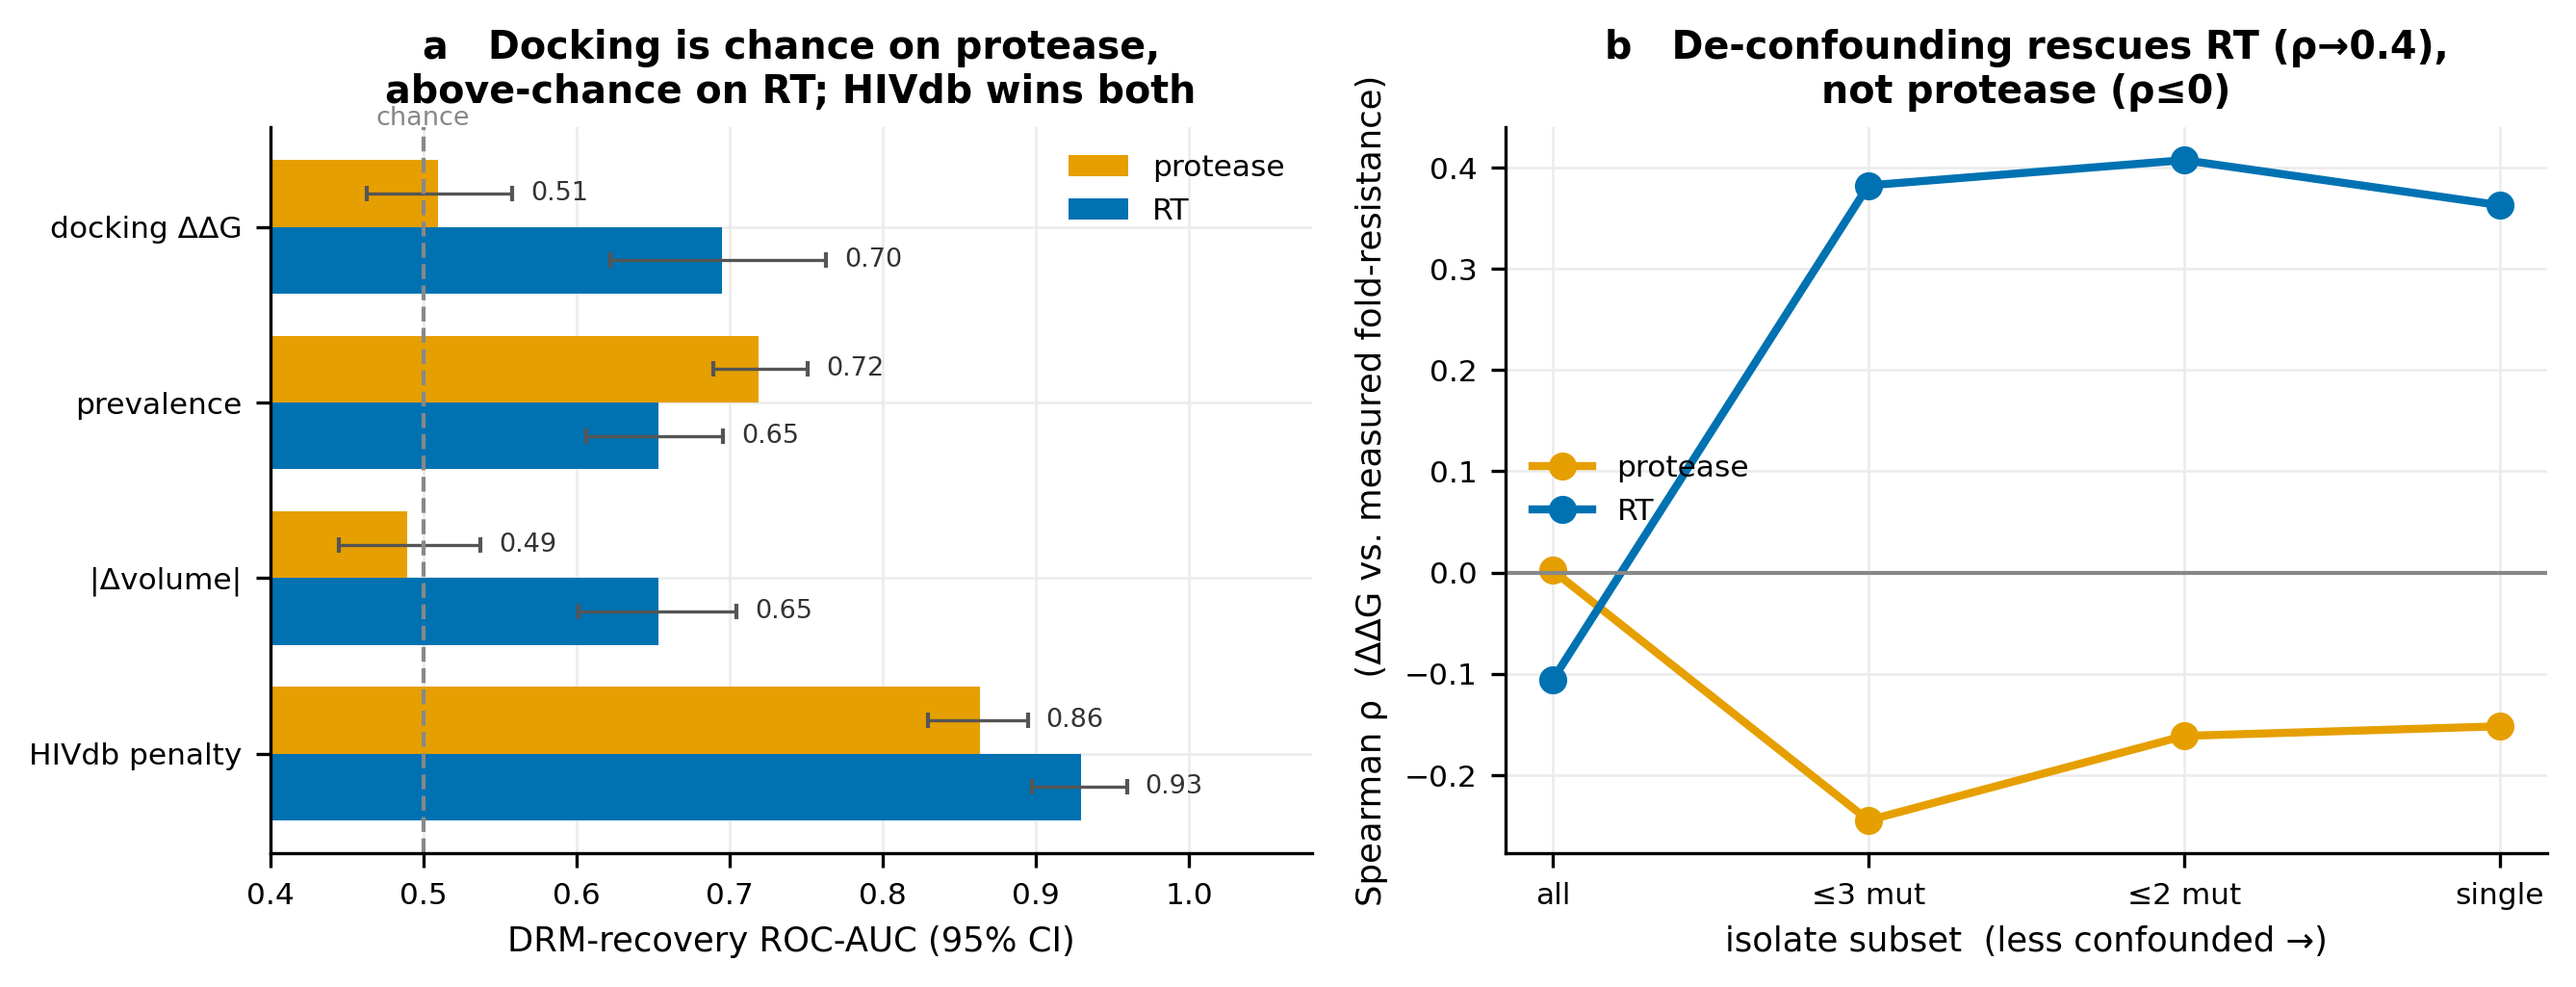
\includegraphics[width=\linewidth]{figures/fig2_benchmark.png}
\caption{\textbf{The predictive benchmark is target-dependent.} (a) DRM-recovery ROC-AUC with bootstrap 95\% CIs: docking-\ddg{} sits on the chance line for protease (0.51) but above it for RT (0.70); the HIVdb expert system wins both. (b) De-confounding: as the fold-resistance target is rebuilt from progressively less co-mutated isolates, RT's magnitude correlation climbs to $\rhoo \approx 0.4$ while protease stays $\leq 0$.}
\label{fig:benchmark}
\end{figure}

\section{Attribution ablation figures}
\label{app:interp}

\begin{figure}[h]
\centering
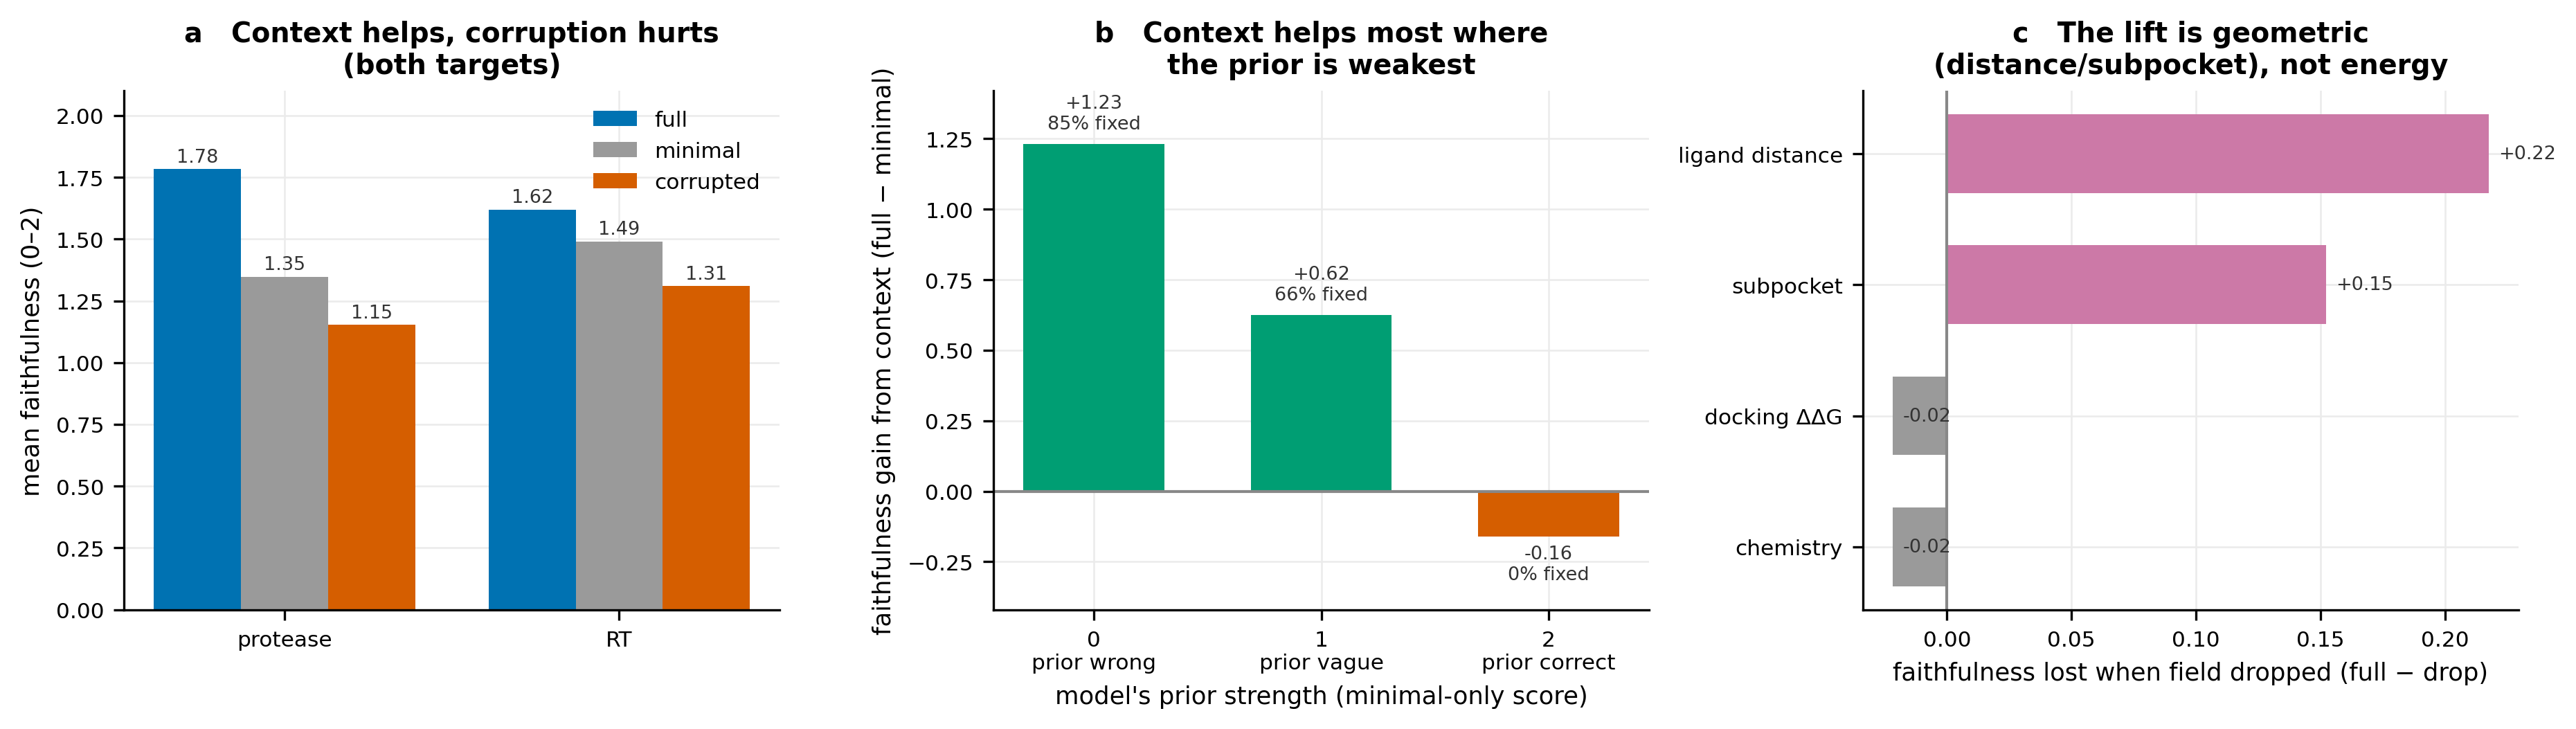
\includegraphics[width=\linewidth]{figures/fig3_interpretability.png}
\caption{\textbf{Attribution ablation.} (a) Faithfulness under full / minimal / corrupted context, both targets: context helps, corruption hurts. (b) The benefit of correct context (full $-$ minimal) by the model's prior strength: largest where the prior alone is wrong (11 of 13 such cases corrected), zero where the prior is already correct. (c) Field-level ablation: the lift comes from geometry (ligand distance, subpocket), not the docking energy or the physicochemistry.}
\label{fig:interp}
\end{figure}

\section{Per-drug breakdown and precision@\texorpdfstring{$k$}{k}}
\label{app:perdrug}

Table~\ref{tab:perdrug} gives the per-drug metrics behind the pooled numbers in
\S4.1, and Table~\ref{tab:patk} the decision-relevant precision@$k$. Both are
produced by \texttt{scripts/14\_precision\_at\_k.py}.

Precision@$k$ ranks a \emph{single} drug's own mutation panel by predicted \ddg{}
(descending, matching the pooled enrichment convention) and reports how many of
the top $k$ are known major DRMs. Significance is an exact one-sided
hypergeometric test---the probability that drawing $k$ mutations at random from
that drug's panel yields at least as many DRMs---which is appropriate at $k=5$
where a bootstrap CI is uninformative.

The per-drug view shows the pooled result is not an artifact of averaging. Every
NNRTI clears its base rate by a wide margin at every $k$; among the PIs only
atazanavir ($k=5$) and lopinavir ($k=20$) reach $p<0.05$, and indinavir---whose
ROC-AUC of 0.388 is \emph{below} chance---returns no DRMs in its top 10. The
protease failure is therefore not uniform noise: it is one target on which the
method is, for some drugs, actively anti-correlated with the truth.

\begin{table}[h]
\centering
\caption{\textbf{Per-drug metrics.} DRM-recovery ROC-AUC and magnitude Spearman \rhoo{} vs.\ measured fold-resistance, per drug. $n$ is the drug's docked panel size, $n_{\text{DRM}}$ its number of major DRMs.}
\label{tab:perdrug}
\begin{tabular}{llrrrrr}
\toprule
target & drug & $n$ & $n_{\text{DRM}}$ & base rate & ROC-AUC & \rhoo{} \\
\midrule
protease & ATV & 258 & 33 & 0.128 & 0.533 & $-0.058$ \\
protease & DRV & 209 & 30 & 0.144 & 0.462 & $0.033$ \\
protease & IDV & 282 & 33 & 0.117 & 0.388 & $-0.085$ \\
protease & LPV & 278 & 33 & 0.119 & 0.552 & $-0.013$ \\
protease & NFV & 284 & 33 & 0.116 & 0.615 & $0.009$ \\
protease & SQV & 280 & 33 & 0.118 & 0.672 & $0.138^{*}$ \\
\midrule
RT & EFV & 423 & 30 & 0.071 & 0.738 & $0.078$ \\
RT & ETR & 301 & 30 & 0.100 & 0.589 & $-0.003$ \\
RT & NVP & 421 & 29 & 0.069 & 0.769 & $0.188^{**}$ \\
RT & RPV & 124 & 25 & 0.202 & 0.634 & $0.126$ \\
\bottomrule
\end{tabular}
\\[2pt]
{\footnotesize $^{*}p<0.05$, $^{**}p<0.001$ for the Spearman correlation.}
\end{table}

\begin{table}[h]
\centering
\caption{\textbf{Per-drug precision@$k$}, reported as (DRMs recovered)/$k$. ${}^{*}$ marks $p<0.05$ by an exact one-sided hypergeometric test against the drug's own base rate.}
\label{tab:patk}
\begin{tabular}{lcccc}
\toprule
drug & $k=5$ & $k=10$ & $k=20$ & base rate \\
\midrule
\multicolumn{5}{l}{\emph{protease}} \\
\quad ATV & 3/5$^{*}$ & 3/10 & 3/20 & 0.13 \\
\quad DRV & 1/5 & 1/10 & 2/20 & 0.14 \\
\quad IDV & 0/5 & 0/10 & 1/20 & 0.12 \\
\quad LPV & 2/5 & 3/10 & 6/20$^{*}$ & 0.12 \\
\quad NFV & 2/5 & 2/10 & 4/20 & 0.12 \\
\quad SQV & 1/5 & 2/10 & 5/20 & 0.12 \\
\midrule
\multicolumn{5}{l}{\emph{RT}} \\
\quad EFV & 4/5$^{*}$ & 8/10$^{*}$ & 15/20$^{*}$ & 0.07 \\
\quad ETR & 3/5$^{*}$ & 7/10$^{*}$ & 11/20$^{*}$ & 0.10 \\
\quad NVP & 4/5$^{*}$ & 8/10$^{*}$ & 15/20$^{*}$ & 0.07 \\
\quad RPV & 3/5 & 7/10$^{*}$ & 9/20$^{*}$ & 0.20 \\
\bottomrule
\end{tabular}
\end{table}

\section{Worked example: one mutation through the ablation}
\label{app:worked}

To make the attribution ablation concrete, we trace a single pair---indinavir
(IDV) and the protease flap mutation \textbf{M46I}---through all three context
conditions. M46I is the paradigm weak-prior case: an \emph{accessory} mutation
that does not touch the inhibitor.

\textbf{Ground truth} (IAS-USA 2022): \emph{``Met46 is a flap residue that does
not contact the inhibitor directly. M46I is an accessory flap mutation that
alters flap dynamics and closure and compensates for active-site mutations,
broadly contributing to PI resistance.''}

Table~\ref{tab:worked} shows the context each condition receives.

\begin{table}[h]
\centering
\caption{\textbf{Structural context supplied to the model} for IDV/M46I under each condition. \emph{Corrupted} keeps the intrinsic chemistry (volume, hydrophobicity) but deranges the pipeline-derived geometry and energy across pairs.}
\label{tab:worked}
\begin{tabular}{lccc}
\toprule
field & full (real) & minimal & corrupted \\
\midrule
min.\ distance to ligand (\AA)  & 7.0 & --- & 4.1 \\
distance to ligand centroid (\AA) & 14.2 & --- & 10.7 \\
contacts ligand directly        & \textbf{False} & --- & \textbf{True} \\
region                          & \textbf{flap} & --- & \textbf{S2/S2$'$ subpocket} \\
$\Delta$volume (\AA$^3$)        & $+3.8$ & --- & $+3.8$ \\
$\Delta$hydrophobicity          & $+2.6$ & --- & $+2.6$ \\
docking \ddg{} (\kcal)          & $-0.24$ & --- & $+0.66$ \\
\midrule
\textbf{judge score} & \textbf{2} & \textbf{0} & \textbf{0} \\
\bottomrule
\end{tabular}
\end{table}

\textbf{Full context} (score 2). \emph{``The M46I mutation increases
hydrophobicity while maintaining nearly identical volume, subtly altering the
hydrophobic landscape of the flap region 7\,\AA{} from indinavir without directly
contacting it\ldots{} reflects reduced entropic penalty for flap closure and
weakened indirect stabilization of inhibitor binding geometry, characteristic of
flap mutations that achieve resistance through conformational rather than direct
contact mechanisms.''} The judge scored 2: the correct primary mechanism.

\textbf{Minimal context} (score 0). \emph{``The M46I substitution replaces a
larger, flexible methionine with a smaller isoleucine, creating a structural
cavity in the S1 subpocket where indinavir's P1 ligand group normally makes
critical van der Waals contacts\ldots{}''} With only the drug and mutation name,
the model defaults to an active-site packing story and \emph{contradicts} the
documented mechanism.

\textbf{Corrupted context} (score 0). \emph{``\ldots{}isoleucine's shorter
branched aliphatic chain cannot maintain the same contact surface\ldots{}the
$\sim$4\,\AA{} minimum distance suggests the residue is in direct contact with the
ligand\ldots{}destabilizes the inhibitor by approximately 0.66\kcal, particularly
affecting the packing interactions critical for IDV's potency in this
region.''}

The corrupted output is the informative one: the explanation \emph{quotes the
falsified values back}---the 4\,\AA{} distance, the S2/S2$'$ region, the 0.66\kcal{}
energy---and reaches the wrong mechanism because of them. This is direct evidence
that the generated mechanism is conditioned on the pipeline's structural fields
rather than retrieved from the model's prior on a famous mutation name, and it is
the single-instance version of the aggregate result in \S4.3.

\section{Reproducibility}
\label{app:repro}

\textbf{Structures and docking.} Protease: PDB 3OXC, chains A/B, catalytic Asp25
dyad asymmetrically protonated, mutations applied to both chains of the homodimer;
box centre $(5.341, -1.893, 14.179)$, size $22^3$\,\AA. RT: PDB 3V81, p66/p51
heterodimer, NNRTI pocket; box centre $(41.105, 52.332, 49.098)$ (occupancy-weighted
centroid of the chain-A nevirapine ligand---note 3V81 contains a second NVP copy
whose inclusion moves the centroid into empty space), size $24^3$\,\AA. AutoDock
Vina 1.2 (CPU) / Uni-Dock (GPU), \texttt{exhaustiveness} 16, 5 poses retained per
run, best pose scored. Receptors cleaned with PDBFixer; mutants built by point
mutagenesis with a frozen-environment clash-relief minimization of the mutated
side chain only; ligands prepared with RDKit (\texttt{AddHs}, ETKDG) and meeko.
Crystal waters, including the conserved flap water, are stripped.

\textbf{Scale and cost.} 285 protease mutant receptors (1{,}591 drug--mutation
pairs across 6 PIs) and 424 RT mutant receptors (1{,}269 pairs across 4 NNRTIs).
The full RT sweep took 19 minutes on a single A100 80GB with Uni-Dock. One RT DRM
(L100I, an isosteric Leu$\rightarrow$Ile) failed receptor construction and is
excluded. For scale, this is roughly three orders of magnitude cheaper per
mutation than the alchemical free-energy protocol of Hauser et al.~\citep{hauser2018}, which is
the trade the paper is about.

\textbf{Models.} Generation and judging both use \texttt{claude-haiku-4-5}
(\texttt{max\_tokens} 1024 for generation, 512 for judging); larger Claude models
decline HIV-resistance \emph{generation} but not judging, which is why the second
judge (\texttt{claude-sonnet-5}) was available for the cross-model check. Scores
are returned through a forced tool call against a fixed \texttt{report\_score}
schema, so every verdict is machine-readable and no free-text parsing is involved.

\textbf{Judge prompt} (verbatim system prompt): \emph{``You are evaluating whether
an AI-generated explanation of HIV-1 protease drug resistance correctly identifies
the known structural mechanism. Score 0 if the explanation contradicts the known
mechanism, 1 if it is consistent but vague or misses the key interaction, 2 if it
correctly identifies the primary structural basis. Judge only structural/mechanistic
agreement, not writing style, and give a one-sentence justification.''} The enzyme
noun is substituted per target. The judge sees the mutation, the drug, the
ground-truth mechanism and the explanation---never the condition label, the
\ddg, or which system produced the explanation.

\textbf{Statistics.} Permutation tests use 5{,}000 label shuffles and bootstrap
CIs 5{,}000 resamples, seed 0. Enrichment ranks by \ddg{} descending. Paired
ablation contrasts use the one-sided Wilcoxon signed-rank test at the
(drug, mutation) level, which is the appropriate paired non-parametric test for
the bounded, tied, non-Gaussian 0/1/2 score differences we observe; a paired
$t$-test would assume a normality the difference distribution violates.
Precision@$k$ significance is the exact hypergeometric test described in
Appendix~\ref{app:perdrug}. We report many tests without multiplicity correction;
the headline contrasts survive at $p<10^{-3}$.

\textbf{Software.} Python 3.11; pandas 2.2.3, numpy 1.26.4, scipy 1.15.3,
scikit-learn 1.7.0, anthropic 0.74.0; RDKit, OpenMM, PDBFixer, AutoDock Vina and
meeko via conda (\texttt{environment.yml}). The pipeline is reproduced by
\texttt{scripts/01}--\texttt{14} in order; each number in this paper is produced by
a named script, and the mapping is in the repository README.

\end{document}
